
%(BEGIN_QUESTION)
% Copyright 2006, Tony R. Kuphaldt, released under the Creative Commons Attribution License (v 1.0)
% This means you may do almost anything with this work of mine, so long as you give me proper credit

Identify the following filled-system types (be as specific as possible -- each system shown here has a unique identifying name!).

$$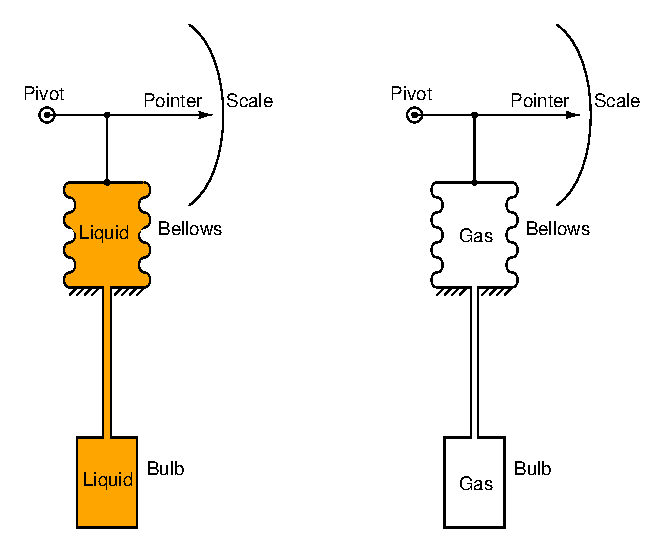
\includegraphics[width=15.5cm]{i00359x01.eps}$$

$$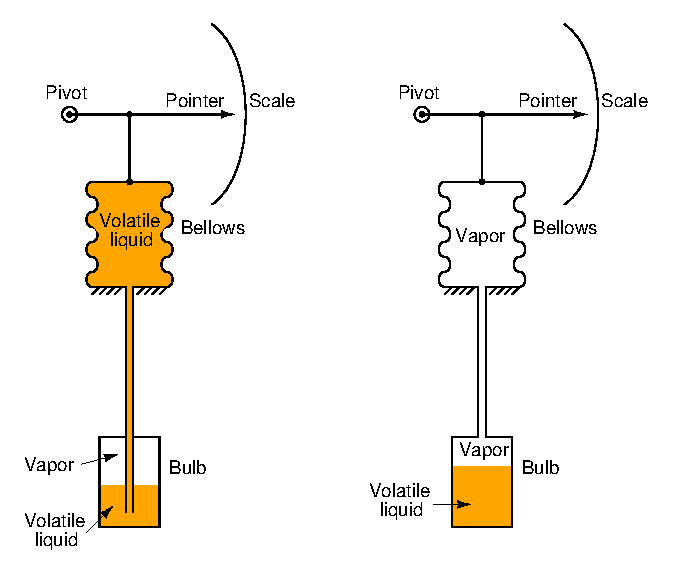
\includegraphics[width=15.5cm]{i00359x02.eps}$$

$$\includegraphics[width=15.5cm]{i00359x03.eps}$$

\underbar{file i00359}
%(END_QUESTION)





%(BEGIN_ANSWER)

$$\includegraphics[width=15.5cm]{i00359x04.eps}$$

$$\includegraphics[width=15.5cm]{i00359x05.eps}$$

$$\includegraphics[width=15.5cm]{i00359x06.eps}$$

\vskip 10pt

Follow-up question: note that a Class IIC system is not shown.  Explain why.

%(END_ANSWER)





%(BEGIN_NOTES)

A Class IIC system switches between Class IIA and Class IIB operation depending on whether the process is warmer than the indicator or vice-versa.

%INDEX% Measurement, temperature: filled-bulb system

%(END_NOTES)


